%% LyX 2.2.3 created this file.  For more info, see http://www.lyx.org/.
%% Do not edit unless you really know what you are doing.
\documentclass[oneside,english]{extbook}
\usepackage{lmodern}
\renewcommand{\sfdefault}{lmss}
\renewcommand{\ttdefault}{lmtt}
\usepackage[T1]{fontenc}
\usepackage[latin9]{inputenc}
\usepackage{geometry}
\geometry{verbose,tmargin=25mm,bmargin=25mm,lmargin=25mm,rmargin=25mm}
\pagestyle{empty}
\setcounter{secnumdepth}{3}
\setcounter{tocdepth}{3}
\setlength{\parindent}{0bp}
\usepackage{babel}
\usepackage{float}
\usepackage{graphicx}
\usepackage{setspace}
\onehalfspacing
\usepackage[unicode=true,pdfusetitle,
 bookmarks=true,bookmarksnumbered=false,bookmarksopen=false,
 breaklinks=false,pdfborder={0 0 1},backref=false,colorlinks=false]
 {hyperref}

\makeatletter
%%%%%%%%%%%%%%%%%%%%%%%%%%%%%% User specified LaTeX commands.
\usepackage{amssymb}
\usepackage{color}
\usepackage{listings}
\definecolor{hellgelb}{rgb}{1,1,0.85}
\definecolor{colKeys}{rgb}{0,0,1}
\definecolor{colIdentifier}{rgb}{0,0,0}
\definecolor{colComments}{rgb}{1,0,0}
\definecolor{colString}{rgb}{0,0.5,0}
\lstset{
      language=Matlab,
      float=hbp,
      basicstyle=\footnotesize\ttfamily,
      identifierstyle=\color{colIdentifier},
      keywordstyle=\color{colKeys},
      stringstyle=\color{colString},
      commentstyle=\itshape\color{colComments},
      columns=fixed,
      tabsize=4,
      frame=single,
      framerule=1pt,
      extendedchars=true,
      showspaces=false,
      showstringspaces=false,
      numbers=left,
      numberstyle=\tiny\ttfamily,
      numbersep=1em,
      breaklines=true,
      breakindent=10pt,
      backgroundcolor=\color{hellgelb},
      breakautoindent=true,
      captionpos=t,
      xleftmargin=1em,
      xrightmargin=\fboxsep
}
\usepackage{lscape}
\usepackage{amsmath}
\usepackage{pifont}
\usepackage{color}

\delimitershortfall=-1pt
\let\Right\right
\let\Left\left
\makeatletter
\def\right#1{\Right#1\@ifnextchar){\!\right}{}}
\def\left#1{\Left#1\@ifnextchar({\!\left}{}}
\makeatother

\makeatother

\begin{document}
\pagenumbering{gobble}

\begin{landscape}
\begin{center}
\textbf{Obstacle's coordinates in the global reference frame}
\par\end{center}

\begin{figure}[H]
\centering\includegraphics[scale=0.95]{/Volumes/HDOC/DOWNLOADS/SCIENCE-ENGINEERING/ROBOTICS/OC-SLAM_AND_PATH_PLANNING/01-GETTING_STARTED/FIGURES/fig03}
\end{figure}

\end{landscape}

\begin{align*}
r \, &= \, \left(Rs \, + \, W \right) \, \alpha\\
l \, & = \, Rs \, \alpha\\
r \, - \, l \, &= \, W \, \alpha
\end{align*}

\begin{align*}
\alpha \, &= \, \dfrac{r \, - \, l}{W}\\
Rs \, &= \, \dfrac{l}{\alpha}
\end{align*}

\begin{align*}
x_l \, &= \, x \, + \, sd \, \cos\left(\theta\right)\\
y_l \, &= \, y \, + \, sd \, \sin\left(\theta\right)
\end{align*}

\begin{align*}
\cos\left(u \, \pm \, v\right) \, = \, \cos u \, \cos v \, \mp \, \sin u \, \sin v\\
\sin\left(u \, \pm \, v\right) \, = \, \sin u \, \cos v \, \pm \, \cos u \, \sin v
\end{align*}

\begin{align*}
\cos\left(\theta \, + \, 90^{\circ}\right) \, &= \,-\,\sin\left(\theta\right)\\
\sin\left(\theta \, + \, 90^{\circ}\right) \, &= \,+\,\cos\left(\theta\right)\\
\end{align*}

\begin{align*}
x_{obs} \, &= \, x_l \, + \, x_{\$} \, + \, x_{\%}\\
         \, &= \, x \, + \, sd \, \cos\left(\theta\right) \, + \, x_* \, \cos\left(\theta\right) \, + \, y_* \, \cos\left(\theta \, + \, 90^{\circ}\right)\\
         \, &= \, x \, + \, sd \, \cos\left(\theta\right) \, + \, D \, \cos\left(\phi\right) \, \cos\left(\theta\right) + D \, \sin\left(\phi\right) \, \cos\left(\theta \, + \, 90^{\circ}\right)\\
         \, &= \, x \, + \, sd \, \cos\left(\theta\right) \, + \, D \, \cos\left(\phi\right) \, \cos\left(\theta\right) - D \, \sin\left(\phi\right) \, \sin\left(\theta\right)\\
         \, &= \, x \, + \, sd \, \cos\left(\theta\right) + D \, \cos\left(\theta + \phi\right)
\end{align*}

\begin{align*}
y_{obs} \, &= \, y_l \, + \, y_{\$} \, + \, y_{\%}\\
         \, &= \, y \, + \, sd \, \sin\left(\theta\right) \, + \, x_* \, \sin\left(\theta\right) \, + \, y_* \, \sin\left(\theta \, + \, 90^{\circ}\right)\\
         \, &= \, y \, + \, sd \, \sin\left(\theta\right) \, + \, D \, \cos\left(\phi\right) \, \sin\left(\theta\right) + D \, \sin\left(\phi\right) \, \sin\left(\theta \, + \, 90^{\circ}\right)\\
         \, &= \, y \, + \, sd \, \sin\left(\theta\right) \, + \, D \, \cos\left(\phi\right) \, \sin\left(\theta\right) + D \, \sin\left(\phi\right) \, \cos\left(\theta\right)\\
         \, &= \, y \, + \, sd \, \sin\left(\theta\right) + D \, \sin\left(\theta + \phi\right)
\end{align*}
\end{document}
